%% LyX 2.2.1 created this file.  For more info, see http://www.lyx.org/.
%% Do not edit unless you really know what you are doing.
\documentclass[12pt,brazil,a4paper]{article}
%\usepackage{sbc-template}
\usepackage[T1]{fontenc}
\usepackage[utf8]{inputenc}
\usepackage{geometry}
\usepackage{graphicx,xcolor,enumerate}
\geometry{verbose,tmargin=2cm,bmargin=2cm,lmargin=2cm,rmargin=2cm}
%\usepackage[linesnumbered,ruled,vlined,portuguese]{algorithm2e}
\usepackage{listings}
\usepackage{amssymb}

% Definições para pseudocódigo
% (necessário acrescentar acentos no literate,
% pois listings não suporta nativamente UTF-8)
\lstdefinelanguage{algo}{
  keywordstyle=[1]{\keywordstyle},
  keywordstyle=[2]{\operatorstyle},
  keywordstyle=[3]{\typestyle},
  keywordstyle=[4]{\functionstyle},
  identifierstyle={\identifierstyle},
  keywords=[1]{%
    início,fim,%
    programa,procedimento,função,subrotina,%
    enquanto,faça,para,até,próximo,repita,até,loop,continue,%
    se,então,senão%
    retorna},
  literate={-}{$-$}1 {^}{$^\wedge$}1
           {>}{{$>$\ }}1 {<}{{$<$\ }}1
           {>=}{{$\geqslant$\ }}1 {<=}{{$\leqslant$\ }}1 
           {:=}{{$\gets$\ }}1 {!=}{{$\ne$\ }}1 {<>}{{$\ne$\ }}1
           {->}{{$\;\to\;$}}1
           {&&}{{\keywordstyle and\ }}4 {{||}}{{\keywordstyle or\ }}3
           {;}{\hspace{0.2em};}2 {,}{\hspace{0.2em},}2
  {á}{{\'a}}1 {é}{{\'e}}1 {í}{{\'i}}1 {ó}{{\'o}}1 {ú}{{\'u}}1
  {Á}{{\'A}}1 {É}{{\'E}}1 {Í}{{\'I}}1 {Ó}{{\'O}}1 {Ú}{{\'U}}1
  {à}{{\`a}}1 {è}{{\`e}}1 {ì}{{\`i}}1 {ò}{{\`o}}1 {ù}{{\`u}}1
  {À}{{\`A}}1 {È}{{\'E}}1 {Ì}{{\`I}}1 {Ò}{{\`O}}1 {Ù}{{\`U}}1
  {ä}{{\"a}}1 {ë}{{\"e}}1 {ï}{{\"i}}1 {ö}{{\"o}}1 {ü}{{\"u}}1
  {Ä}{{\"A}}1 {Ë}{{\"E}}1 {Ï}{{\"I}}1 {Ö}{{\"O}}1 {Ü}{{\"U}}1
  {â}{{\^a}}1 {ê}{{\^e}}1 {î}{{\^i}}1 {ô}{{\^o}}1 {û}{{\^u}}1
  {ã}{{\~a}}1 {õ}{{\~o}}1 
  {Â}{{\^A}}1 {Ê}{{\^E}}1 {Î}{{\^I}}1 {Ô}{{\^O}}1 {Û}{{\^U}}1
  {œ}{{\oe}}1 {Œ}{{\OE}}1 {æ}{{\ae}}1 {Æ}{{\AE}}1 {ß}{{\ss}}1
  {ű}{{\H{u}}}1 {Ű}{{\H{U}}}1 {ő}{{\H{o}}}1 {Ő}{{\H{O}}}1
  {ç}{{\c c}}1 {Ç}{{\c C}}1 {ø}{{\o}}1 {å}{{\r a}}1 {Å}{{\r A}}1
  {€}{{\euro}}1 {£}{{\pounds}}1 {«}{{\guillemotleft}}1
  {»}{{\guillemotright}}1 {ñ}{{\~n}}1 {Ñ}{{\~N}}1 {¿}{{?`}}1
}

\lstset{%
  language={algo},
  columns=fullflexible,
  numbers=left,
  numberstyle=\scriptsize,
  mathescape=true,
  xleftmargin=.04\textwidth
}

% Ajustes de estilos
\newcommand\keywordstyle{\rmfamily\bfseries\upshape}
\newcommand\operatorstyle{\rmfamily\mdseries\upshape}
\newcommand\typestyle{\rmfamily\mdseries\upshape}
\newcommand\functionstyle{\rmfamily\mdseries\scshape}

\newcommand\identifierstyle{\rmfamily\mdseries\itshape}

% Comandos para incluir mais palavras reservadas,
% operadores, tipos e funções/procedimentos

\newcommand\addkeywords[1]{%
  \lstset{morekeywords=[1]{#1}}}

\newcommand\addoperators[1]{%
  \lstset{morekeywords=[2]{#1}}}

\newcommand\addtypes[1]{%
  \lstset{morekeywords=[3]{#1}}}

\newcommand\addfunctions[1]{%
  \lstset{morekeywords=[4]{#1}}}
  
\RequirePackage{times}
\makeatletter

\newenvironment{code}
{\par\begin{list}{}{
\setlength{\rightmargin}{\leftmargin}
\setlength{\listparindent}{0pt}% needed for AMS classes
\raggedright
\setlength{\itemsep}{0pt}
\setlength{\parsep}{0pt}
\normalfont\ttfamily}%
 \item[]}
{\end{list}}

\setlength{\jot}{0.25\jot}
\usepackage{latexsym}

\makeatother

\usepackage{babel}
\begin{document}

\title{Algoritmo de Simulação de Book de Ofertas de Ações}

\author{Cassiano Luis Flores Michel, Leonardo Vargas Schilling\\
Ciência da Computação — PUCRS\\
Algoritmos e Estruturas de Dados 2 - Marcelo Cohen}

\date{17 de setembro de 2021}
\maketitle

\vspace{3cm}

\begin{center}

\includegraphics[width=10cm]{logo_pucrs.png}

\end{center}

\vspace{10cm}

\section*{Introdução}

\hspace{0.5cm}Neste artigo busca-se descrever o processo de criação de um algoritmo para leitura de um arquivo de texto, onde simula-se o recebimento de uma ordem de compra ou venda de ações a cada linha.\vspace{0.4cm}

A cada linha lida, devem-se realizar todas as operações possíveis até aquele momento, através das seguintes regras:

\begin{enumerate}
\item A empresa não realiza preguízo (Preço de compra > Preço de venda);
\item A empresa prioriza a maior diferença entre Preço de Compra e Venda;
\item A empresa lucra com a diferença entre os valores de compra e venda;
\item A primeira linha do arquivo indica o número de operações.

\end{enumerate}

\begin{center}
\textit{Formato da linha do arquivo:} \medskip

\textit{<operação> <quantidade> <preço>} \medskip

\textit{Exemplo:} \medskip

\textit{C 129 14} \medskip
\textit{V 302 12}
\end{center}

\section*{Estratégia}

\hspace{0.5cm} Entende-se que para atingir o seu objetivo, as ordens de \textbf{compra} devem ser ordenadas por preço \textit{decrescente}, enquanto as ordens de \textbf{venda} devem ser ordenadas por preço \textit{crescente}. \medskip

Desta forma a operação com maior lucro para a empresa sempre será através da execução da primeira ordem de venda e da primeira ordem de compra da coleção. \medskip

Para cada linha lida, insere a operação na coleção e executa as operações possíveis, por fim, imprime os resultados analisados:

\begin{enumerate}
\item Lucro;
\item Tempo de execução aproximado;
\item Total de operações aproximado;
\item Ordens de compra não executadas;
\item Ordens de venda não executadas;
\item Nome do arquivo.

\end{enumerate}

\vspace{2cm}

\section*{Estruturas de dados}

\hspace{0.5cm} Optou-se por utilizar implementações \textit{opensource} de filas de prioridade através de heaps binários. Um heap binário é uma estrutura de dados baseada em árvores binárias que satisfaz sempre a propriedade de heap, que diz que se o nó B é filho do nó A, então a chave de A é maior ou igual a chave de B. \vspace{1cm}

\textbf{Demonstração de um Min Heap e Max Heap}

\begin{center}
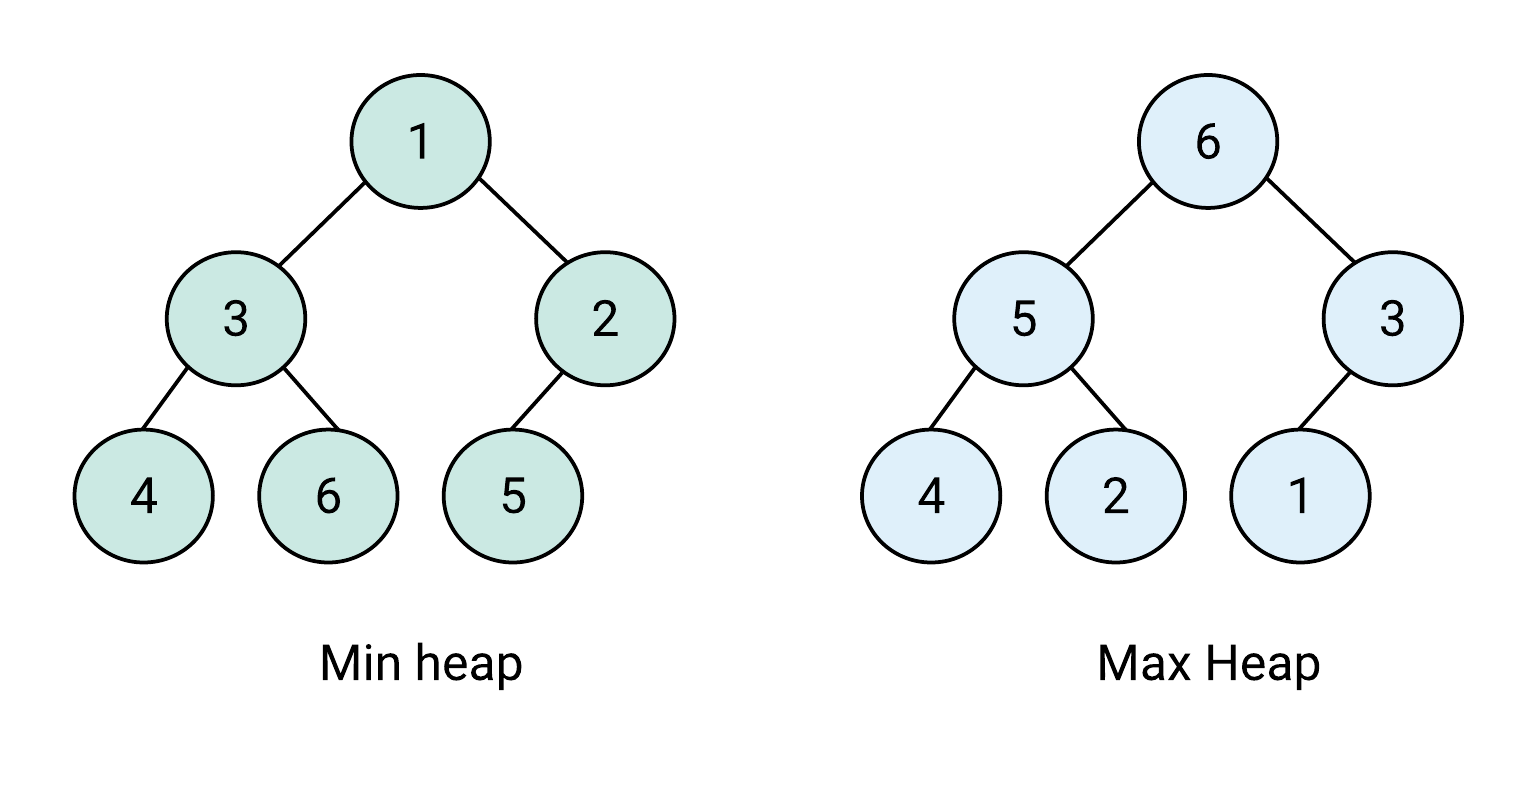
\includegraphics[width=10cm]{figura_1.png}

\tiny Fonte: https://medium.com/@rohan04/easy-way-to-implement-the-heap-data-structure-in-python-5658d0a6d266
\end{center}

\bigskip
\section*{Algoritmo}

\hspace{0.5cm} A complexidade de tempo para a inserção (executada N vezes, sendo N o número de linhas do arquivo – 1) é O(log n); \medskip

O acesso ao valor máximo ou mínimo dos heaps (valor que será checado para validar se existem operações lucrativas a serem executadas) é O(1); \medskip

Caso haja uma operação lucrativa a ser executada (se o preço da raiz do minheap for menor ou igual ao preço da raiz do maxheap), executam-se as ordens possíveis; \medskip
	
Ao executar determinada ordem, caso a quantidade de compra ou venda das ordens prioritárias vire zero, então a ordem é removida (através do método delMin ou delMax) com complexidade O(log n); \medskip

Serão executadas N inserções (em O(log n)), e até N remoções (considerando um cenário onde uma ordem de compra executa todas as ordens de venda ou vice-versa) portanto, pode-se considerar a complexidade do algoritmo como O(n log n). \vspace{7cm}

\textbf{Fluxograma}

\begin{center}
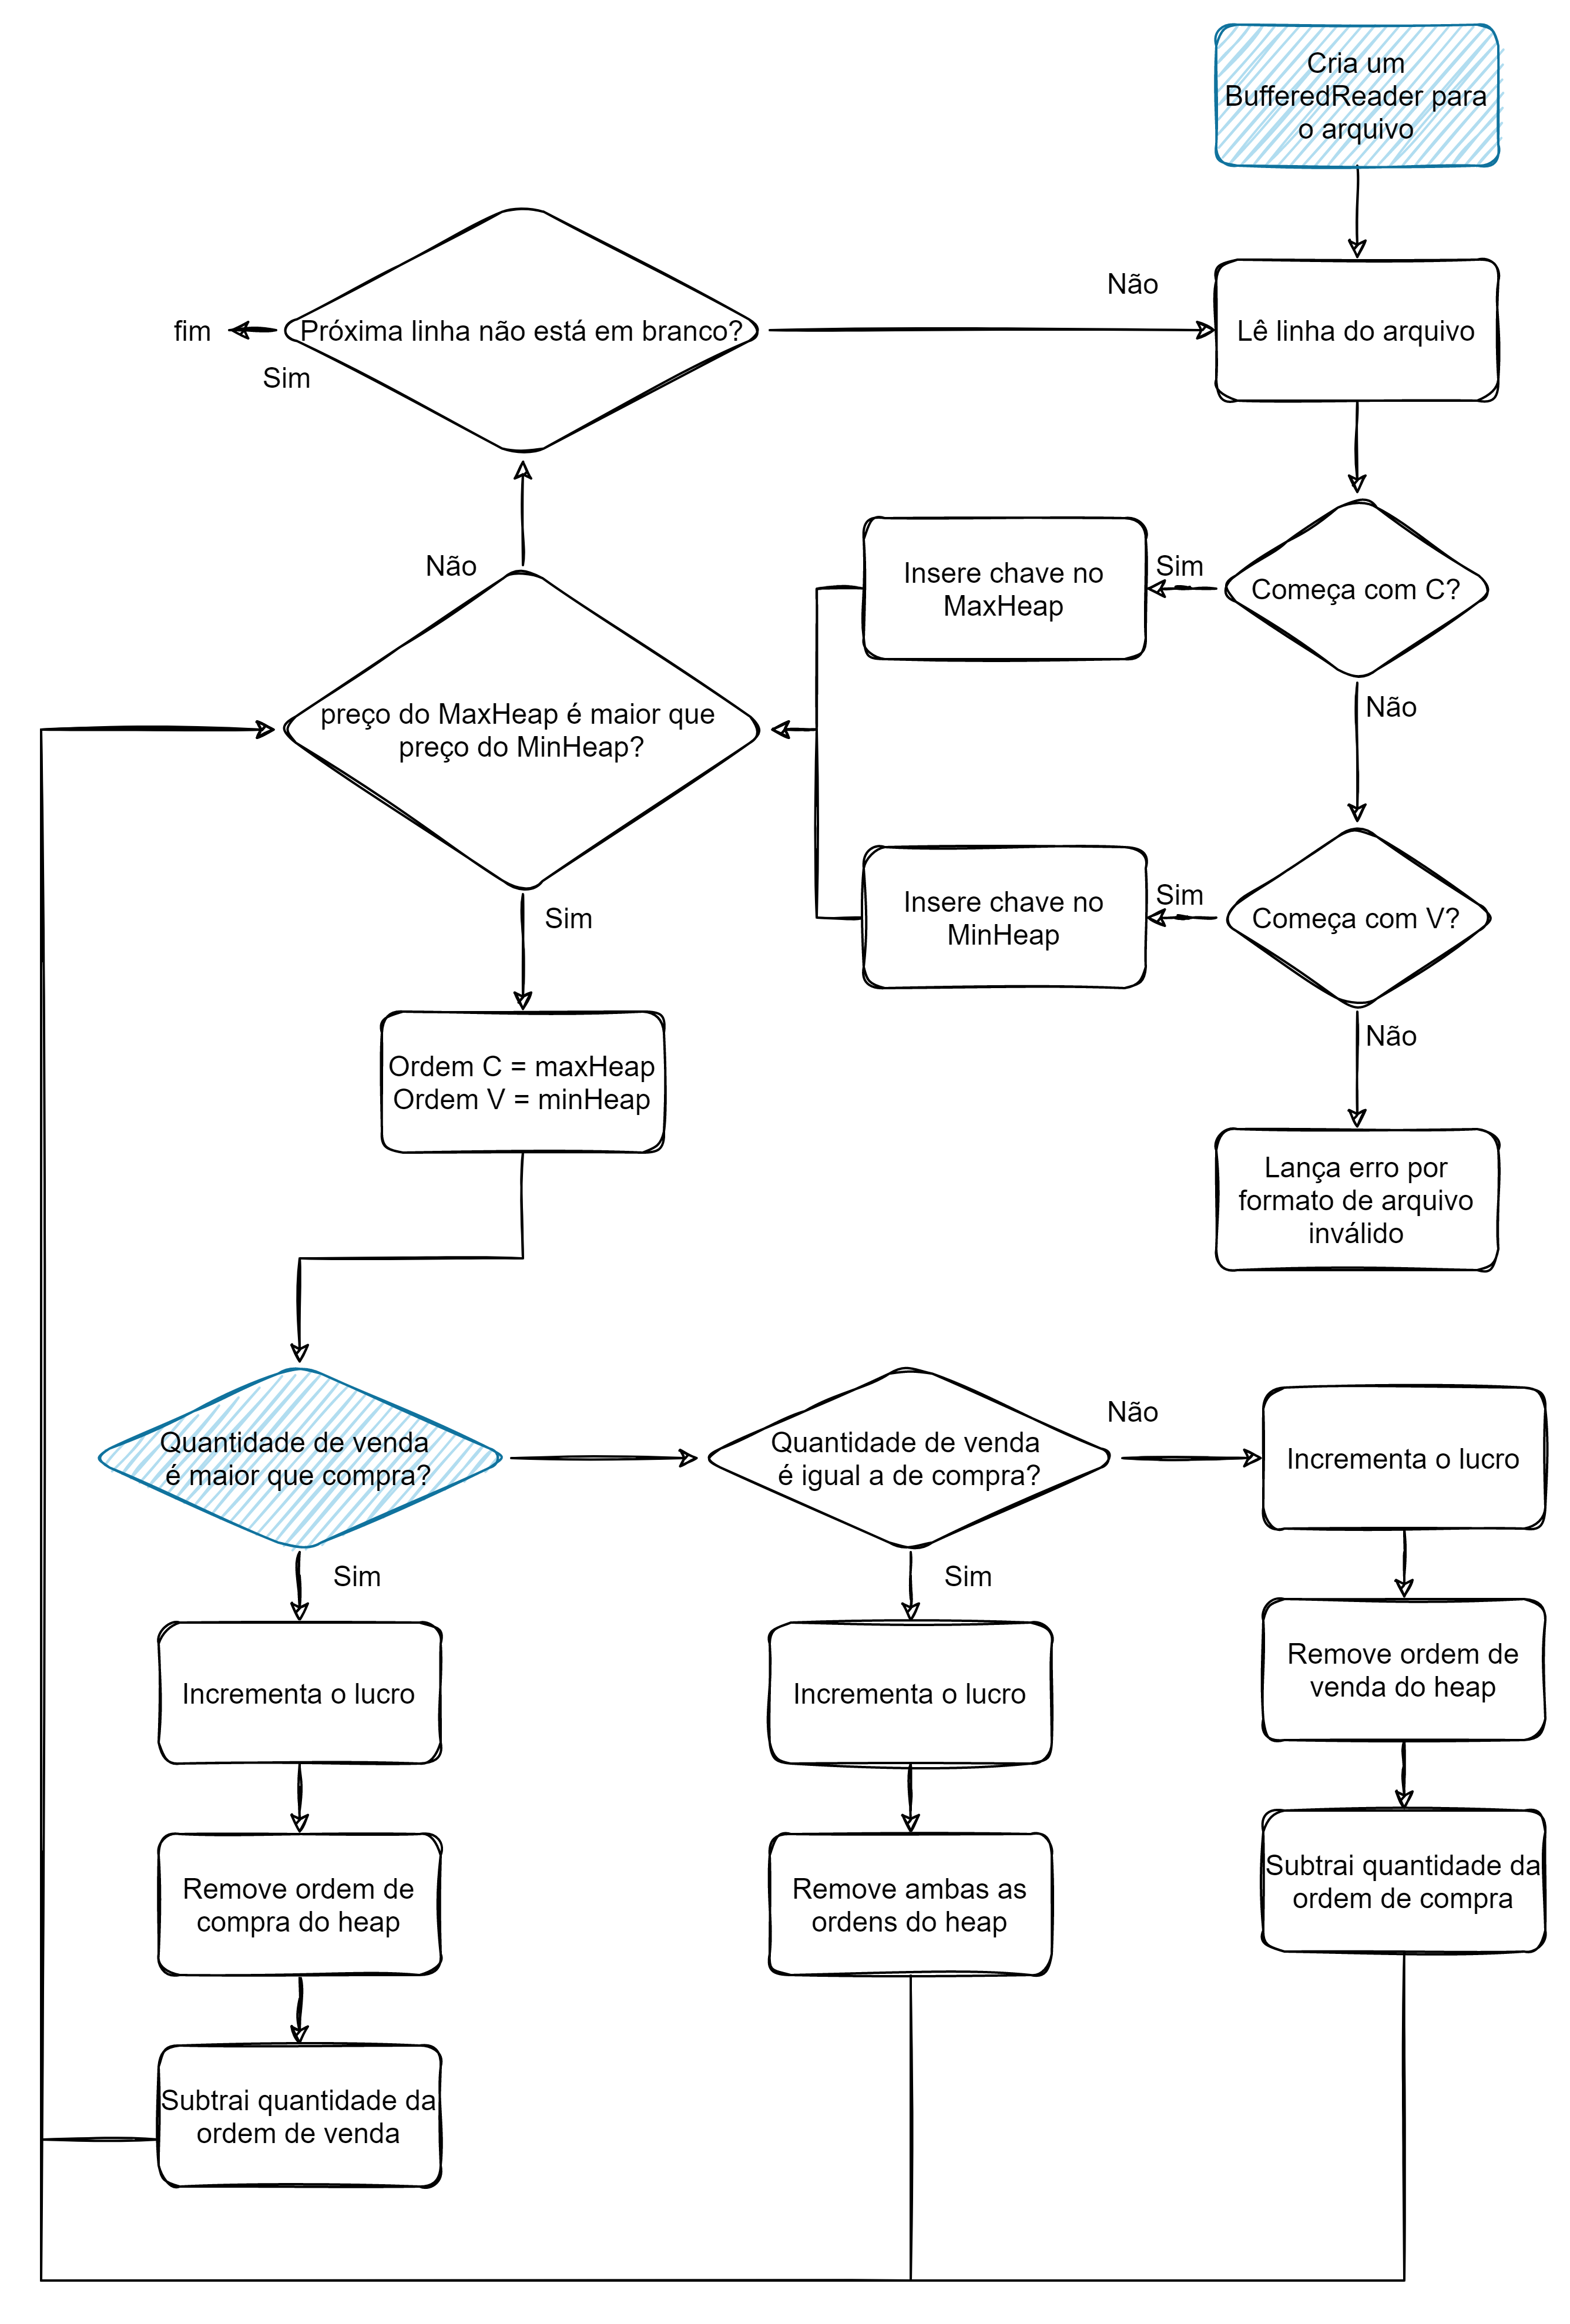
\includegraphics[width=14cm]{figura_2.png}

\end{center}
\vspace{3cm}

\section*{Resultados}

\hspace{0.5cm}Após a execução do algoritmo com todos os casos de teste, os dados foram tratados no Excel, para análise do tempo de operação e número de operações. \medskip

A contagem de operações se deu através da criação de uma classe \textbf{Contador}, cujo atributo \textit{count} foi incrementado em todos os trechos e iterações do fluxo \textit{(inserção, remoção, sink, swim, assertHeap)}. \vspace{0.7cm}

\begin{center}
\textbf{Tabela de Resultados} \vspace{0.5cm}

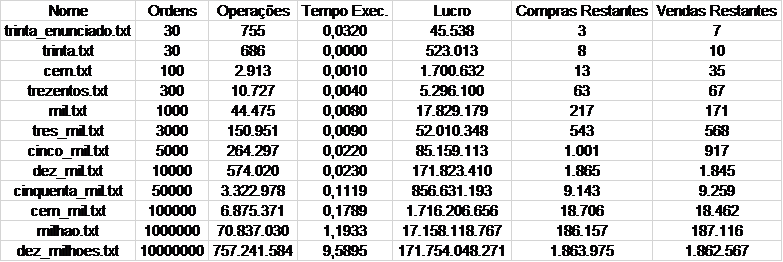
\includegraphics[width=16cm]{figura_3.png}
\vspace{0.1cm}

\small Fonte: os autores

\end{center}

\vspace{0.5cm}
\hspace{0.3cm} Com os dados de tempo de execução, número de operações e número de ordens (linhas do arquivo de texto), foi possível esboçar dois gráficos:

\vspace{0.5cm}

\begin{center}
\textbf{Número de Operações x Número de Linhas do Arquivo} \vspace{0.5cm}

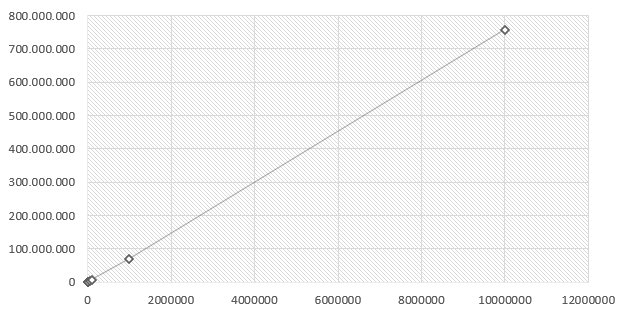
\includegraphics[width=16cm]{figura_4.png}
\vspace{4cm}

\textbf{Tempo de Execução (s) x Número de Linhas do Arquivo} \vspace{0.5cm}

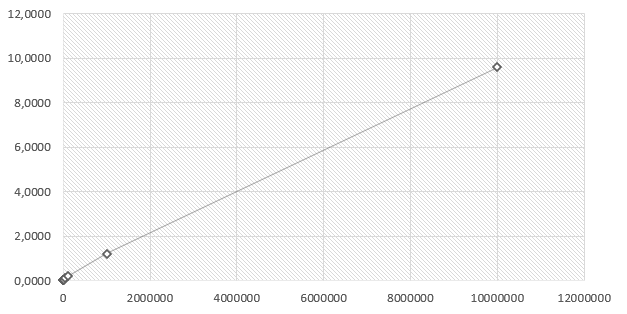
\includegraphics[width=16cm]{figura_5.png}
\vspace{0.1cm}
    
\end{center}

\vspace{15cm}

\begin{thebibliography}{1}
\vspace{0.5cm}

\bibitem{1} Sedgewick, Robert; Wayne, Kevin: ``\textbf{Priority Queues}''. Last modified on December 29, 2017. Available in: https://algs4.cs.princeton.edu/24pq

\bibitem{2} Rohan: ``\textbf{Easy way to implement the Heap data-structure in Python.}''. Last modified on July 17, 2020. Available in: https://medium.com/@rohan04/easy-way-to-implement-the-heap-data-structure-in-python-5658d0a6d266

\end{thebibliography}

\end{document}